\section{Wahrscheinlichkeit}
\begin{table}[H]
	\centering
	\begin{tabular}{l|l}
		Alle Versuchsausgänge & $\Omega$ \\
		A und B treten ein & $A \cap B$ \\
		A oder B treten ein & $A \cup B$ \\
		nicht A & $\overline{A} = \Omega \backslash A$ \\
		unmögliches Ereignis & $\emptyset$ \\
		A hat B zurfolge & $A \subset B$ \\
	\end{tabular}
\end{table}

\textbf{Axiome}:\\
\begin{align*}
	P(\emptyset) &= 0 \\
	P(\overline{A}) &= P(\Omega \backslash A) = 1 - P(A) \\
	P(A \backslash B) &= P(A) - P(A \cap B) \\
	P(A \cup B) &= P(A)  + P(B) - P(A \cap B) \\
	P(\overline{A} | \overline{B}) &= 1-P(A|\overline{B}) \\
	P(\overline{A} | B) &= 1-P(A|B) \\
\end{align*}

\subsection{Bedingte Wahrscheinlichkeit}
Die bedingte Wahrscheinlichkeit eines Ereignisses A unter der Bedingung B. \textit{B ist die neue Gesammtmenge, in welcher A vorkommen kann}:
\[
P(A|B) = \frac{P(A \cap B)}{P(B)} \xRightarrow[\text{S.v. Bayes}]{} P(A|B) = P(B|A)\cdot\frac{P(A)}{P(B)}
\]

\noindent\textbf{Beispiel:} Die Wahrscheinlichkeit, dass ein Raucher (R) Lungenkrebs (L) einwickelt ist $15\%$, Bei Nichtraucher $1\% \rightarrow P(L|R) = 0.15$ und $P(L|\overline{R}) = 0.01$. Wie viel Lungenkrebskrange sind auch Raucher ist unbekannt $P(R|L) = ?$.

\noindent Wenn A und B unabhängig sind gilt:
\[ P(A \cap B) = P(A) \cdot P(B)\]


\subsection{Totale Wahrscheinlichkeit}
Vollständig abgeschlossene Menge von $m$ paarweisen disjunkten Ereignissen, dann gilt:
\[
P(A) = \sum_{n=0}^{m}P(A\cap B_m) = \sum_{n=0}^{m}P(A|B_n)\cdot P(B_n)
\]

\noindent\textbf{Beispiel}
\begin{align*}
	P(A) &=P(A|B)P(B) + P(T|\overline{B})P(\overline{B}) \\
	&= P(A|B)P(B) + (1 - P(\overline{A}|\overline{B}))P(\overline{B})
\end{align*}

\subsection{Statistische Kennwerte}
\subsubsection{Leistung}
Zweites Moment: statistische Leistung kann als statische Gesamtleistung aufgefasst werden
\[
E(X^2) = \int_{-\infty}^{\infty}x^2\cdot f_X(x)dx
\]

\subsubsection{Erwartungswert}\script{60}
Der Erwartungswert $\mu$ einer Zufallsvariable beschreibt die Zahl, die die diese im Mittel annimmt.
\[
\mu = \overline{X} = E(X)= \sum\limits_{i=0}^{n}x_i\cdot \underbrace{P(X=x_i)}_\text{Wr.keit} = \int_{-\infty}^{\infty}x\cdot \underbrace{\varphi(x)}_{\text{Wr.dichte}}dx
\]

\textbf{Rechenregeln} mit Zufallsvariablen $X, Y$:
\begin{itemize}[nosep]
	\item $E(X + Y) = E(X) + E(Y)$
	\item $E(\lambda X) = \lambda E(X)$ 
	\item $E(X\cdot Y) = E(X) \cdot E(Y) \qquad$  (Nur falls Unabhängig)
\end{itemize}

\subsubsection{Varianz}
Die Varianz $\var(X)$ beschreibt die mittlere quadratische Abweichung vom Erwartungswert. Damit lässt sich die Standardabweichung $\sigma$ berechnen.
\begin{align*}
	\var(X) &= E(X^2) - E(X)^2 \\
	&=\sum\limits_{i=0}^{n}(k_i - E(X))^2 \cdot \underbrace{P(X=x_i)}_\text{Wr.keit} \\
	\sigma &= \sqrt{\var(X)}	
\end{align*}

\noindent\textbf{Beispiel} Faire Münze:\\
$P(X = \overbrace{0}^{k_1}) = \frac{1}{2}$, Kopf: $P(X = \overbrace{1}^{k_2}) = \frac{1}{2}$ und der Erwartungswert $E(X)$: 
\begin{align*}
	E(X) &= 0\cdot \frac{1}{2} + 1\cdot\frac{1}{2} = \frac{1}{2} \\
	E(X^2) &= 0^2\cdot \frac{1}{2} + 1^2\cdot\frac{1}{2} = \frac{1}{2}
\end{align*}

\noindent Die Varianz kann auf zwei Arten berechnet werden:\\
\textit{Option1:} $\var(X) = (0 - \frac{1}{2})^2 \cdot \frac{1}{2} + (1 - \frac{1}{2})^2 \cdot 1 \xrightarrow{} \frac{1}{4}$\\
\textit{Option2:} $\var(X) = E(X^2) - E(X)^2 = \frac{1}{2} - \frac{1}{4} \rightarrow \frac{1}{4}$
\\ ~\\
\noindent\textbf{Rechenregeln}:
\begin{itemize}[nosep]
	\item $\var(\lambda X) = \lambda^2\var(X)$
	\item $\var(X + Y) = \var(X) + \var(Y) \qquad$ (Nur falls Unabhängig)
	\item $\var(X\cdot Y) = \var(X)\var(Y) + \var(Y)E(X)^2 + \var(X)E(Y)^2$
\end{itemize}

\subsubsection{Kovarianz}
Eine positive Kovarianz gibt an, dass sich beide Variablen in dieselbe Richtung bewegung und dual. Werte nahe oder gleich Null, deuten darauf hin, dass die Zufallsvariablen unabhängig sind. Wenn $\cov(x, y) = 0$, sind sie unkorreliert. In Nachrichtentechnik ist die DC-bereinigte statistische Kreuzleistung und zeigt die Ähnlichkeit von X und Y bzgl. Abweichung vom Mittelwert auf.

Die Kovarianz zwischen Zufallszahl $x,y$ mit Mittelwerten $\overline{x}, \overline{y}$ wird wie folgt berechnet.

\[
\cov(x,y) = \frac{\sum\limits_{i=1}^{N}(x_i - \overline{x})(y_i - \overline{y})}{N} = E(xy) - E(x)\cdot E(y)
\]

\subsubsection{Korrelationskoeffizient}
Korrelationskoeffizient ist ein normiertes Mass der Kovarianz. $\left|\textbackslash{}varphi\_\{xy\}\right| \leq 1$.
\[
\varphi_{xy} = \varphi(x, y) = \frac{\sigma_{xy}}{\sigma_x \cdot \sigma_y}
\]

\subsection{Wahrscheinlichkeitsverteilungen}
\subsubsection{Wahrscheinlichkeitsdichte}
Die Fläche zwischen einem Punkt $a$ und $b$ zeigt die Wahrscheinlichkeit an. Nicht der Wert von der Wahrscheinlichkeitsdichtefunktion ist somit relevant, sondern die Fläche unter ihrm Graphen. Die Wahrscheinlichkeitsdichte muss daher auch den Flächeninhalt $1$ haben. 
\[
\int_{-\infty}^{\infty}\varphi(x)dx = 1
\]

\subsubsection{Verteilungsfunktion}
Die Verteilungsfunktion $F$ gibt an, mit welcher Wahrscheinlichkeit das Ergebnis des Zufallsexperiments kleiner oder gleich eines bestimmten Wertes ist. Dafür werden alle Ergebnisse bis zu diesem Wert summiert. 
\[
\varphi(x) = F'(x) \xRightarrow[]{} \int_{-\infty}^{x}\varphi(\zeta)d\zeta = F_x(x)
\]
$F$ ist die Stammfunktion von der Wahrscheinlichkeitsdichte $\varphi$.

\subsubsection{Gleichverteilung}
Gleichverteilung liegt zB vor wenn Zufallszahlen  in einem Intervall von $[a, b]$ gleichverteilt sind. Jede Zahl sollte gleich Wahrscheinlich vorkommen. Der Erwartungswert kann einfach durch $E(X) = \frac{a + b}{2}$ bestimmt werden. für Varianz gilt $\var(x) = \frac{(b-a)^2}{12}$
\[
\varphi(x) = \begin{cases}
	0 & x < a \\
	\frac{1}{b-a} & x \in [a,b] \\
	0 & x > b
\end{cases}
\]


\subsubsection{Binomialverteilung}
Zufallsexperiment mit zwei möglichen Ausgängen $A$ oder $\overline{A}$ zB Lotto, Wahrscheinlichkeit $p = P(A)$. $X$ = Anzahl Eintreten von $A$ in $n$ unabhängigen Durchführungen. Der Erwartungswert kann auch durch $E(X) = np$ und die Varianz $\var(X) = np(1 - p)$ berechnet werden.
\[
P(X = k) = \underbrace{\begin{pmatrix}	n \\ k \end{pmatrix}}_{\text{Anzahl Auswahl}}\cdot \underbrace{p^k}_{\text{Eintreten von A}}\cdot\underbrace{(1-p)^{n-k}}_{\text{Eintreten von }\overline{A
}}
\]
\noindent\textbf{Beipsiel:} Wie gross ist die Wahrscheinlichkeit, dass bei 10 Würfen einees fairen Würfels 7 mal die 5 kommt. Das Einzelereignis ist $p = P(\text{Augenzahl } 5) = \frac{1}{6}$
\[
P (X = 7) = \begin{pmatrix}	10 \\ 7 \end{pmatrix} \frac{1}{6^7}\begin{pmatrix}	5 \\ 6 \end{pmatrix}^3 = 0.000248
\]

\textbf{Approximation Normalverteilung}\\
Für grosse $n$ und eher grosse $p$ kann die Binomialverteilung auch mit der Standard- Normalverteilung approximiert werden. Damit werden $\mu = np$ und $\sigma = \sqrt{np(1-p)}$ standardisierte. \textbf{Achtung:} für die Grenzen immer $\pm 0.5$ addieren, um Rundungsfehler zu minimieren.
\begin{align*}
	P(X \leq k) &\approx \Phi(\frac{k + 0.5 - \mu}{\sigma}) \\
	P(l < X \leq k) &\approx \Phi(\frac{k + 0.5 - \mu}{\sigma})  - \Phi(\frac{k - 0.5 - \mu}{\sigma}) \\
\end{align*}

\textbf{Approximation Poissonverteilung}\\
Für grosse $n$ und eher kleine $p$ wird die Binomialverteilung besser mit der Poissonverteilung approximiert. $\lambda = np$
\[
P_\lambda(k) = e^{-\lambda}\frac{\lambda^k}{k!}
\]


\subsubsection{Normalverteilung}
Summe vieler kleiner Einflüsse wie Messwerte oder wiederholte Experimente. Zwei Drittel aller Werte liegen innerhalb einer Standardabweichung $\sigma$ um den Erwartungswert $\mu$. Diese Verteilung wird verwendet, wenn $P$ irgendwo in der mitte liegt, für seltene (kleine $P$) kann die Piossonverteilung verwendet werden.
\[
\varphi(x) = \frac{1}{\sigma\sqrt{2\pi}}e^{-\frac{(x-\mu)^2}{2\sigma^2}}
\]
\noindent Die Varianz ist zudem gegeben durch die Wendestellen bei $\mu \pm \sigma \rightarrow \var(x) = E(X^2) - E(X)^2 = \sigma^2E\left(\frac{(x - \mu)^2}{\sigma^2}\right)$

\begin{center}
	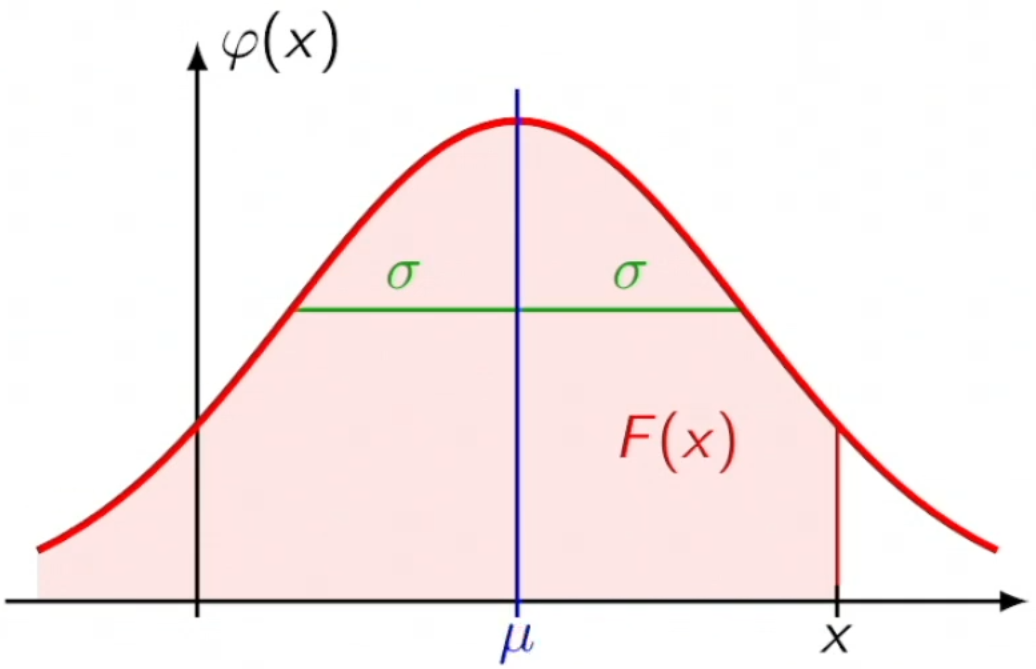
\includegraphics[width=0.4\columnwidth]{Images/normalverteilung}
\end{center}

\noindent Wenn die Normalverteilung Standardisiert wurde, kann die Tabelle verwendet werden. $\Phi(-x) = 1 - \Phi(x)$


\textbf{erf Fehelerfunktion} \script{145} und \script{259}
$\erf(x)$ bezieht sich auf eine Normalverteilung mit $\mu = 0$ und $\sigma = \frac{1}{\sqrt{2}}$\\
	\[
\erf(\xi) = \frac{2}{\sqrt{\pi}}\cdot\int_{0}^{\xi}e^{-x^2}dx
\]


\textbf{Q Funktionen} \script{146} und \script{261}
$\erf(x)$ bezieht sich auf eine Normalverteilung mit $\mu = 0$ und $\sigma = 1$\\
	\[
Q(\xi) = \frac{1}{\sqrt{2\pi}}\cdot\int_{\xi}^{\infty}e^{\frac{-x^2}{2}}dx
\]

\subsubsection{Poissonverteilung}
Gedächnislose Prozesse $T_i$ mit gleichem $a$. Wobei $k$ die Anzahl der Prozesse und $\lambda = al$ mit $l$ der Länge auf dem Intervall ist. $\lambda$ kann auch eine Rate sein. \textbf{Achtung:} Dies sollte nur verwendet werden, wenn $n$ gross und $P$ selten ist.
\[
P_k(\lambda) = e^{-\lambda}\frac{\lambda^k}{k!}
\]
